\section{V64 Interferometrie}
\label{sec:V64}

\begin{itemize}
    \item Ziel ist die Bestimmung der Brechungsindices von Luft/Kohlenstoffdioxid/Glas
        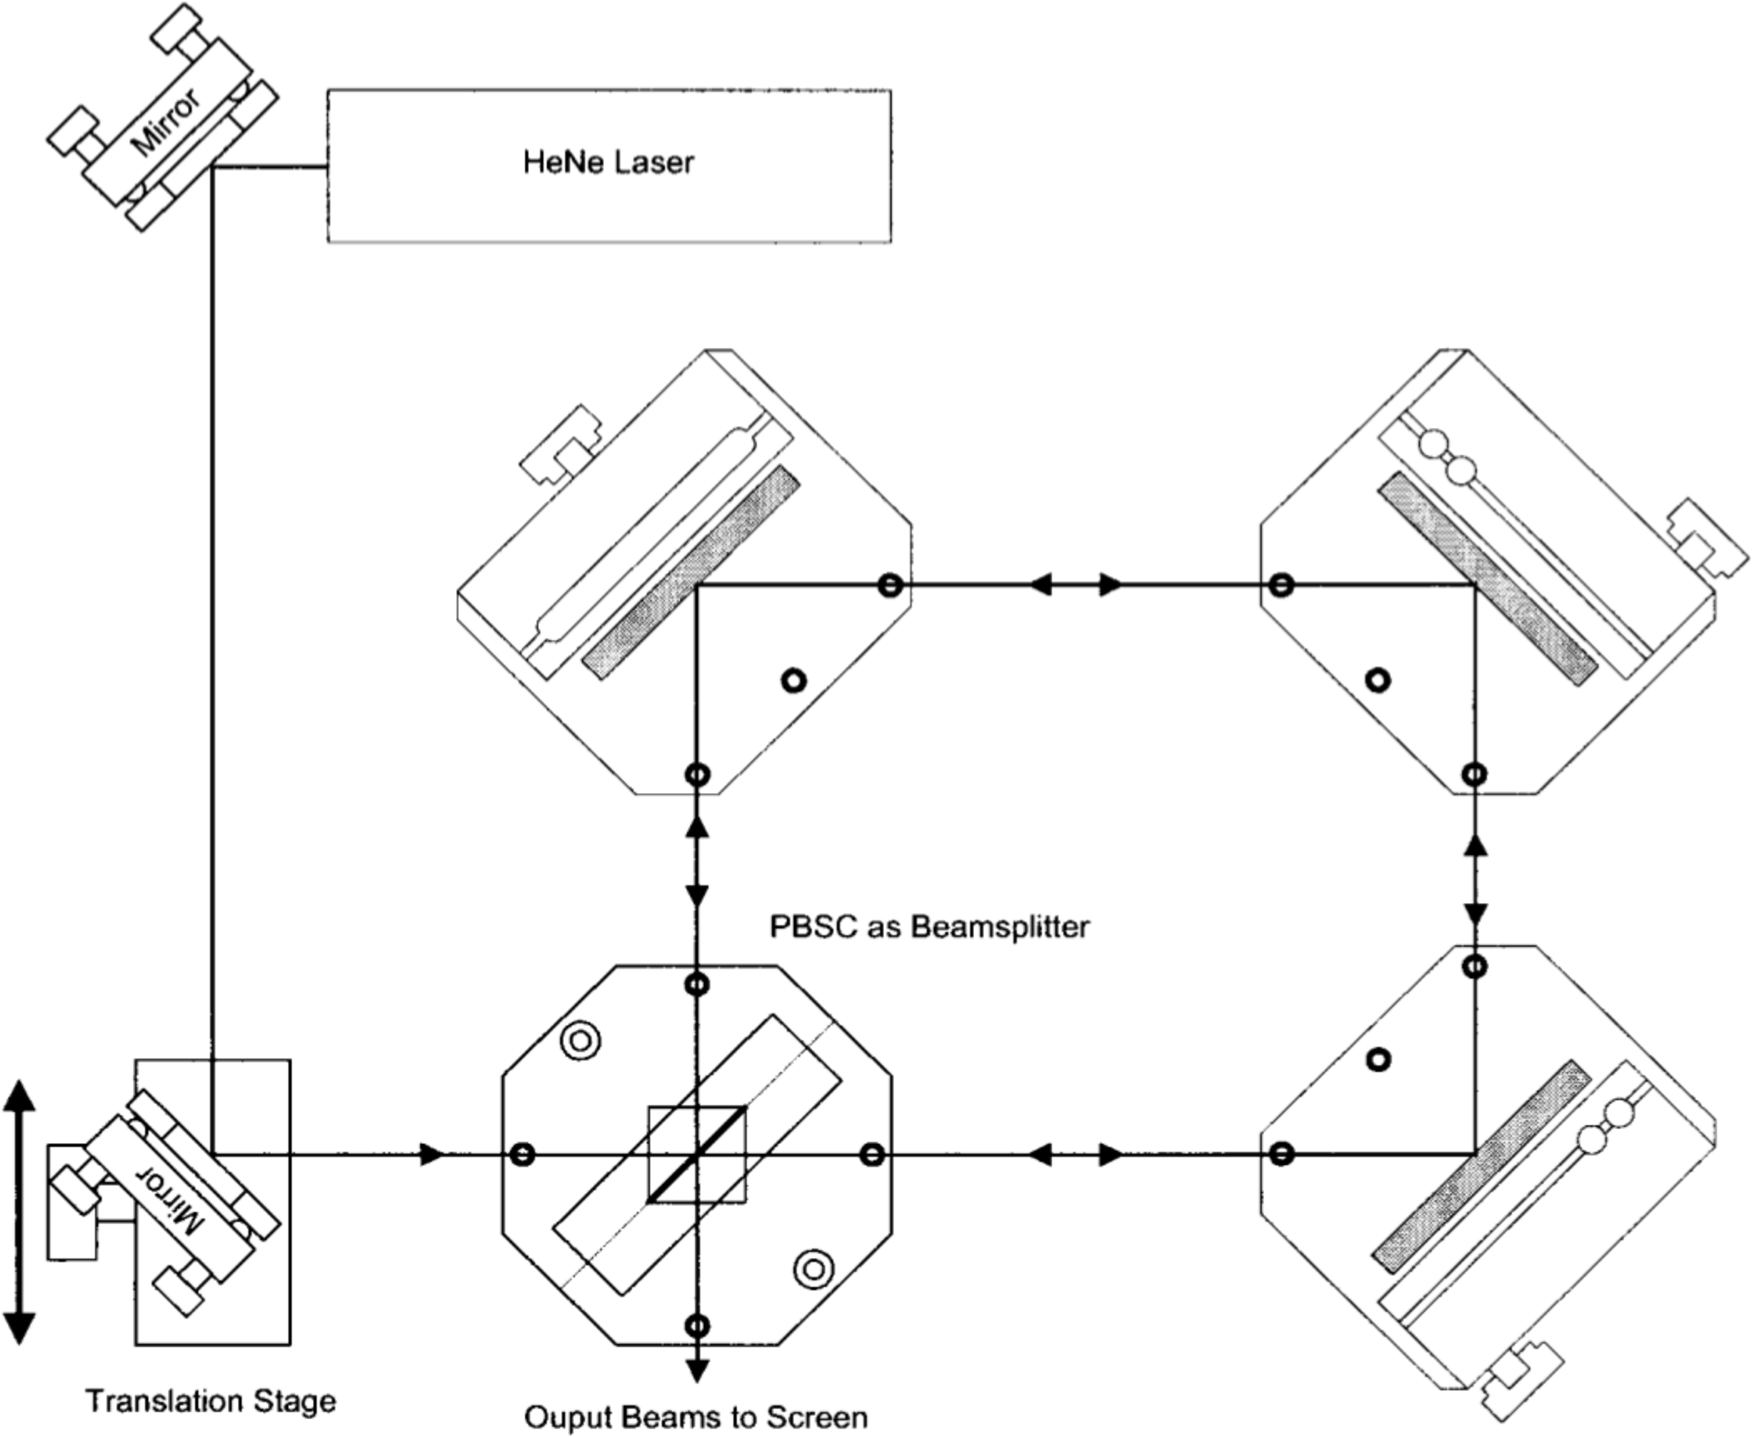
\includegraphics[width=0.6\textwidth]{figures/sagnac.pdf}
    \item Sagnac-Interferometer: HeNe-Laser Strahl $\SI{632,8}{\nano\meter}$ über zwei Spiegel in Interferometer
    \item trifft dann auf polarisierenden Strahlteiler: Ein Teil passiert geradlinig, ein Teil rechtwinklig reflektiert
    \item senkrecht zueinenader polarisiert
    \item Strahlteiler: zwei Prismen mit dreieckiger Grundfläche, Strahl trifft im 45grad Winkel auf Grenzfläche
    \item Strahlen laufen dann über drei Spiegel im Rechteck, wobei Überlagerung
    \item dann erneut auf den Strahlteiler und reflektiert zu PM
    \item leichtes Verschieben des zweiten Spiegels ermöglicht Tennen in zwei Teilstrahlen innerhalb der Apparatur
    \item so kann etwas in den einen Strahl gelegt werden, ohne den anderen zu beeinflussen
    \item Vorteil dieses Aufbaus: resistent gegen kleiner Erschütterungen, da beide Strahlen den selben Weg durchlaufen
    \item \textbf{Kontrast:} $K=\frac{I_\text{max}-I_\text{min}}{I_\text{max}+I_\text{min}}$, zwischen 1 und 0
    \item hier: Untersuchung des Kontrastes in Abhängigkeit des Polarisationswinkels eines Filters
    \item $K\propto |\sin(2\varphi+\delta)|$
    \item Brechungsindex in Materie ist Quotient der Lichtgeschwindigkeit im Vgl. zum Vakuum
    \item Phasendifferenz zwischen Strahlen durch Gaszelle in einem Strahl
        \begin{equation}
            \upD\varphi = \frac{2\pi}{\lambda_\text{vac}}\upD n
        \end{equation}
    \item linearer Zusammenhang zwischen Phasendifferenz und Brechungsindexdifferenz
    \item Zusammenhang zwischen Anzahl Intensitätsmaxima und Brechungsindex $M = \frac{\upD\varphi}{2\pi}$
    \item Brechungsindex $n = \frac{\lambda_\text{vac}}{L}M +1$
    \item Im Allgemeinen ist $n$ aber druck- und temperaturabhängig (Lorentz-Lorenz-Gleichung)
        \begin{equation}
            \frac{n^2-1}{n^2+2} = \frac{Ap}{RT}
        \end{equation}
    \item für Gase ist $n$ i.d.R. etwa 1, sodass man vereinfachen kann zu $n\approx \sqrt{1+\frac{3Ap}{RT}}$
    \item Bei Festkörper, wo nicht einfach Druck oder Temperatur variiert werden können, kann die Wegstrecke über die Drehung geometrisch verändert werden
    \item \textbf{Allgemein was zu Brechung etc}
\end{itemize}

\textbf{Durchführung}
\begin{itemize}
    \item erst Kontrastbestimmung: Polarisationsfilter vor Interferometer und von 0 bis 360grad variiert
    \item Messe Photostrom in Abängigkeit vom Winkel und bestimme som Maximum/Minimum (daraus Kontrast)
    \item wiederholt sich in $\pi$
    \item $n_\text{Glas}$: zehnmal den Winkel des Doppelglashalters langsam von 0 bis $\SI{10}{\degree}$ drehen
    \item Zählautomatik misst dabei Anzahl der Interferenzmaxima
    \item $n_\text{gas}$: Evakuierung und Ventilierung der Gaszelle je drei Messreihen in Abh. des Drucks
    \item $\SI{50}{\milli\bar}$ Schritte von $\SI{50}{\milli\bar}$ bis $\SI{1000}{\milli\bar}$
    \item aus der Regression: $m\approx\frac{3A}{2RT}$, dann auf Normalbedingungen umrechnen ($\frac{T}{T_0}$)
\end{itemize}
